% Uncomment this to make slides with overlays:
\documentclass[slides]{beamer}

% Uncomment these (but comment the above \documentclass line) to make handouts:
%\documentclass[handout]{beamer}

% Uncomment these to have more than one slide per page
%\usepackage{pgfpages}
%\pgfpagesuselayout{2 on 1}[border shrink=5mm]
%\pgfpageslogicalpageoptions{1}{border code=\pgfusepath{stroke}}
%\pgfpageslogicalpageoptions{2}{border code=\pgfusepath{stroke}}

\usepackage[]{graphicx, color, hyperref}

\mode<presentation>
{
	%\usetheme[secheader]{Boadilla}
	%\usecolortheme[rgb={.835, .102,.169}]{structure}  
	\usetheme[width= 0cm]{Goettingen}
	%\setbeamercovered{transparent}
}
\setbeamertemplate{navigation symbols}{}
\setbeamertemplate{footline}[frame number]

\definecolor{blue2}{rgb}{0.278,0.278,0.729} 
\newcommand{\blue}[1]{\textcolor{blue2}{#1}}
\newcommand{\white}[1]{\textcolor{white}{#1}}
\newcommand{\red}[1]{\textcolor{red}{#1}}
\newcommand{\xbar}{\overline{x}}
\newcommand{\ybar}{\overline{y}}
\newcommand{\phat}{\widehat{p}}
\newcommand{\prob}{\mbox{Pr}}
\newcommand{\E}{\mathbb{E}}
\newcommand{\Var}{\mbox{Var}}
\newcommand{\cp}{\oplus}
\newcommand{\cm}{\circleddash}

\title{Lecture 13: Central Limit Theorem + Confidence Intervals}
\author{Chapter 4.4 + 4.2}
\date{}

\begin{document}
%------------------------------------------------------------------------------
\begin{frame}
\titlepage
\end{frame}
%------------------------------------------------------------------------------


%------------------------------------------------------------------------------
\begin{frame}[fragile]
\frametitle{Goals for Today}

\begin{itemize}
\item Discuss the Central Limit Theorem
\item Introduce confidence intervals
\item Interpretation
\end{itemize}

\end{frame}
%------------------------------------------------------------------------------


%------------------------------------------------------------------------------
\begin{frame}[fragile]
\frametitle{Recap}

\begin{itemize}
\item \blue{Point estimates} are based on a sample $x_1, \ldots, x_n$ and are used to estimate population parameters.
\pause \item The \blue{sampling distribution} characterizes the (random) behavior of point estimates (like $\xbar$).
\pause \item The standard deviation of a sampling distribution is the \blue{standard error}: it quantifies the uncertainty/variability of point estimates.  
\end{itemize}

\end{frame}
%------------------------------------------------------------------------------


%------------------------------------------------------------------------------
\begin{frame}[fragile]
\frametitle{Illustrative Image}

\begin{center}
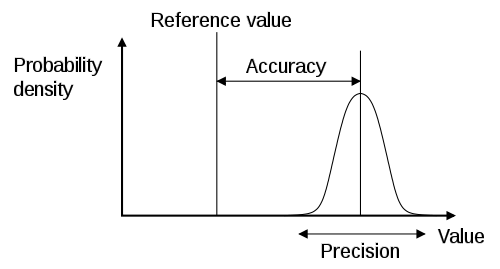
\includegraphics[width=\textwidth]{figure/Accuracy_and_precision.png}
\end{center}

\end{frame}
%------------------------------------------------------------------------------


%------------------------------------------------------------------------------
\begin{frame}
\frametitle{Central Limit Theorem}
\begin{center}
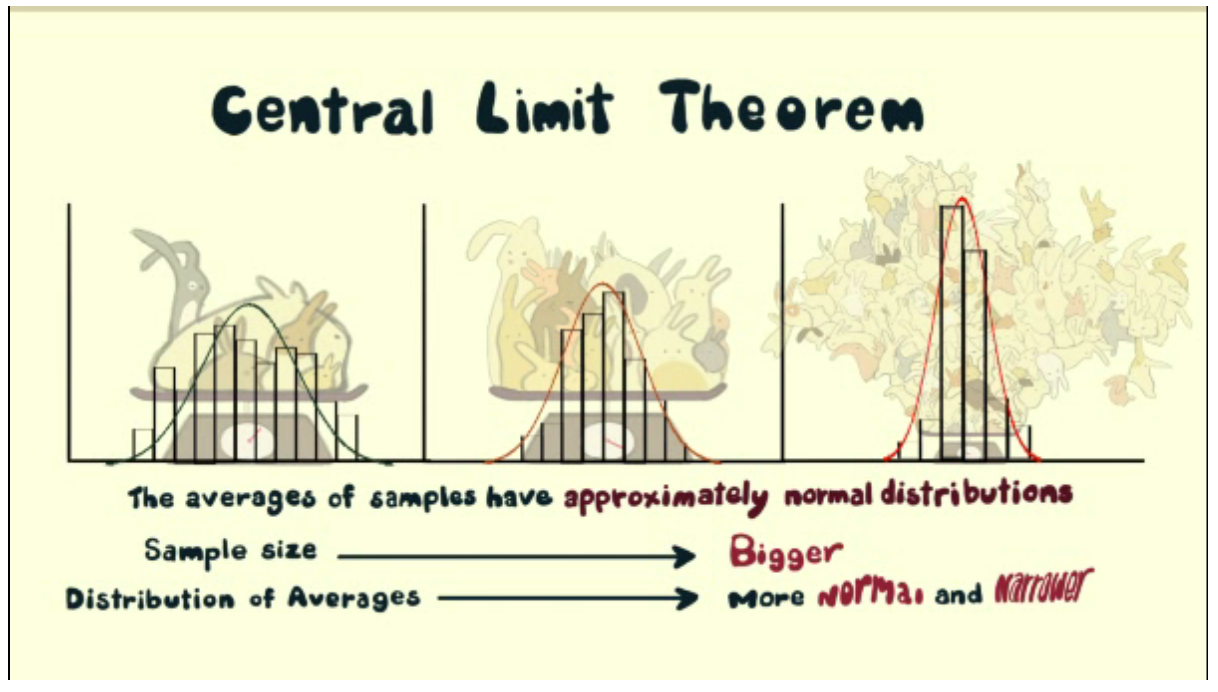
\includegraphics[width=\textwidth]{figure/CLT.png}
\end{center}
\end{frame}
%------------------------------------------------------------------------------


%------------------------------------------------------------------------------
\begin{frame}
\frametitle{Central Limit Theorem}
\blue{Question}:  Why do we care about the CLT?

\vspace{0.25cm}

\pause\blue{Answer}:  We want the sampling distribution of $\xbar$ to be Normal \blue{irregardless} of the shape of population distribution.

\vspace{0.25cm}

\pause\blue{Example}:  The bimodal (population) distribution of dragon wing spans has a mean of 6.5:

\pause\begin{center}
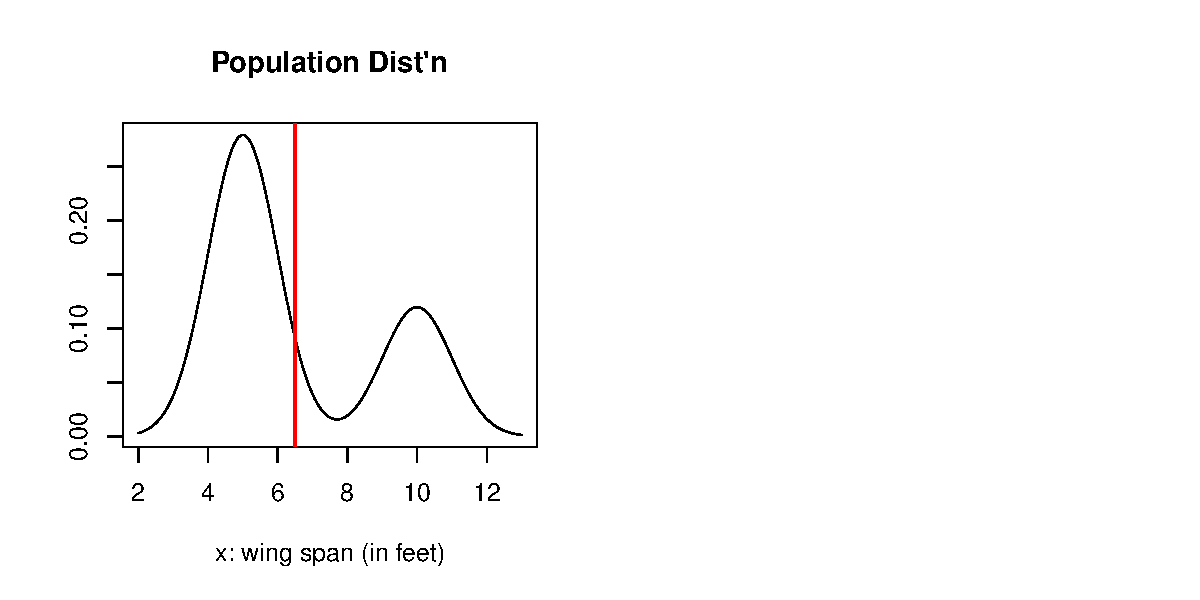
\includegraphics[width=\textwidth]{figure/CLT1.pdf}
\end{center}

\end{frame}
%------------------------------------------------------------------------------


%------------------------------------------------------------------------------
\begin{frame}
\frametitle{Central Limit Theorem}
\blue{Question}:  Why do we care about the CLT?

\vspace{0.25cm}

\blue{Answer}:  We want the sampling distribution of $\xbar$ to be Normal \blue{irregardless} of the shape of population distribution.

\vspace{0.25cm}

\blue{Example}:  The bimodal (population) distribution of dragon wing spans has a mean of 6.5:

\begin{center}
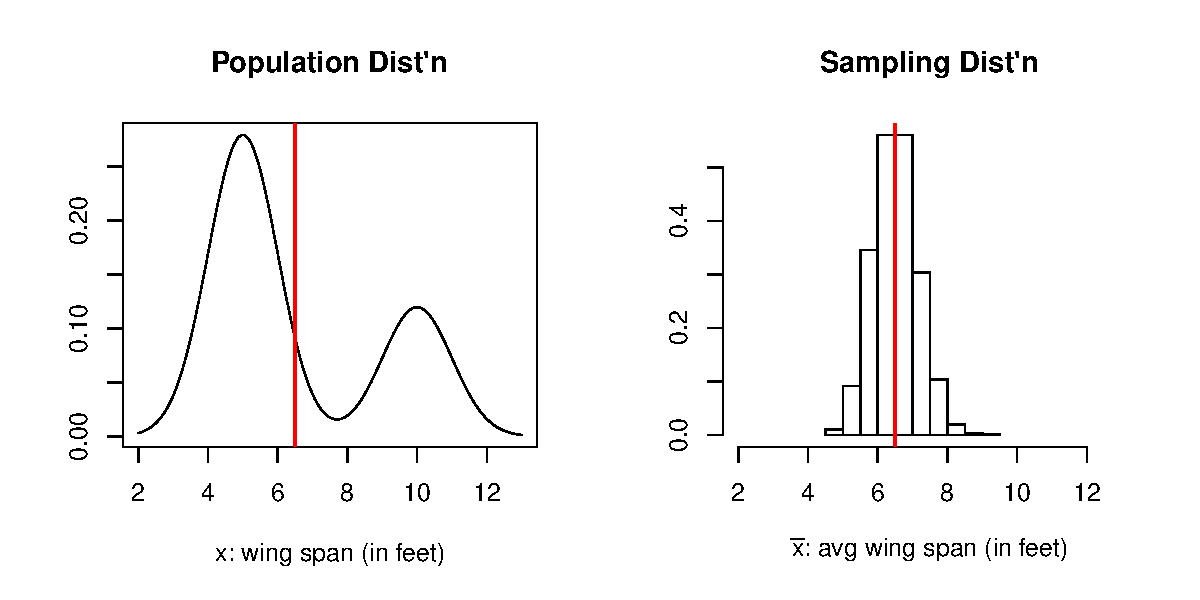
\includegraphics[width=\textwidth]{figure/CLT2.pdf}
\end{center}

\end{frame}
%------------------------------------------------------------------------------


%------------------------------------------------------------------------------
\begin{frame}
\frametitle{Central Limit Theorem}
\blue{Question}:  Why do we care that the sampling distribution of $\xbar$ is Normal?

\vspace{0.25cm}

\pause\blue{Answer}:  So we can use the Normal table on p.409 of the book to calculate probabilities.  We call this using the \blue{normal model}.

\vspace{0.25cm}

\begin{center}
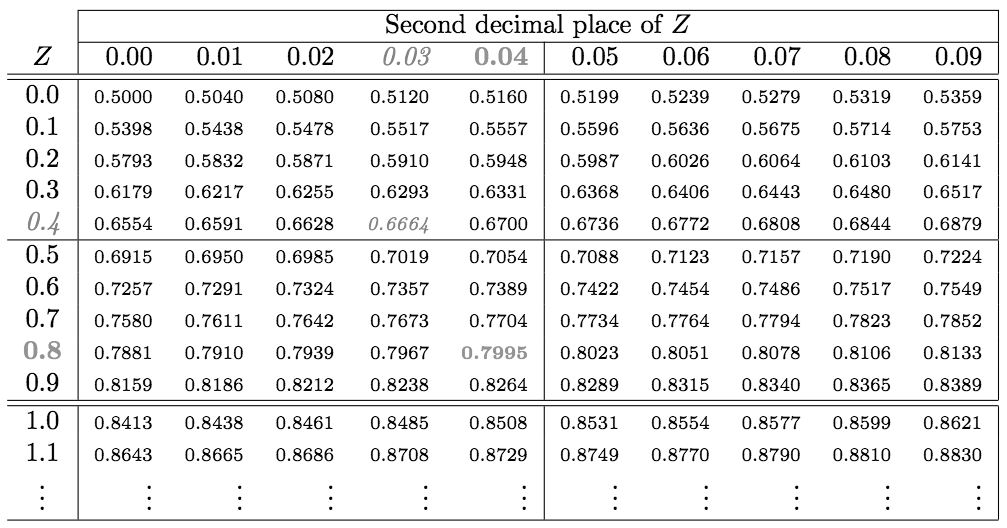
\includegraphics[width=0.7\textwidth]{figure/normal_table.png}
\end{center}


\end{frame}
%------------------------------------------------------------------------------


%-------------------------------------------------------------------------------
\begin{frame}
\frametitle{Definition}

For a sample $x_1, \ldots, x_n$ of \blue{independent} observations, if $n$ is ``large'' enough to counteract the skew of the population distribution, then the sampling distribution of $\xbar$ is approximately Normal with
\begin{itemize}
\item mean $\mu$
\item SD equal to the $SE=\frac{\sigma}{\sqrt{n}}$
\end{itemize}

\vspace{0.25cm}

\pause\blue{Key}:  this holds for any population distribution, not just a normally distributed population.  

\vspace{0.25cm}

\pause \blue{Recall}: If we don't know $\sigma$, we can plug in its point estimate $s$ if the two conditions are satisfied.  


\end{frame}
%-------------------------------------------------------------------------------


%-------------------------------------------------------------------------------
\begin{frame}
\frametitle{Conditions for the Normal Model}

This translates to the following conditions to be able to use the Normal model with $s$ in place of $\sigma$, as stated in the book:

\begin{enumerate}
\pause\item $n\leq$ 10\% of the population size.\\
\pause Comment:  To ensure independence.
\pause\item $n \geq 30$.\\
\pause Comment:  This is a \blue{rule of thumb} that works for most cases.  In some situations you might need less, in others more.
\pause \item The population distribution is not strongly skewed.\\
Comment: This is related to the $n$ necessary.  The larger the $n$, the more lenient we can be with the skew assumption.
\end{enumerate}

\end{frame}
%-------------------------------------------------------------------------------


%------------------------------------------------------------------------------
\begin{frame}
\frametitle{Example of Skew vs $n$}
Let's say your observations come from the following very skewed \blue{population distribution} with mean $\mu=\textcolor{red}{0.011109}$. 
\begin{center}
\pause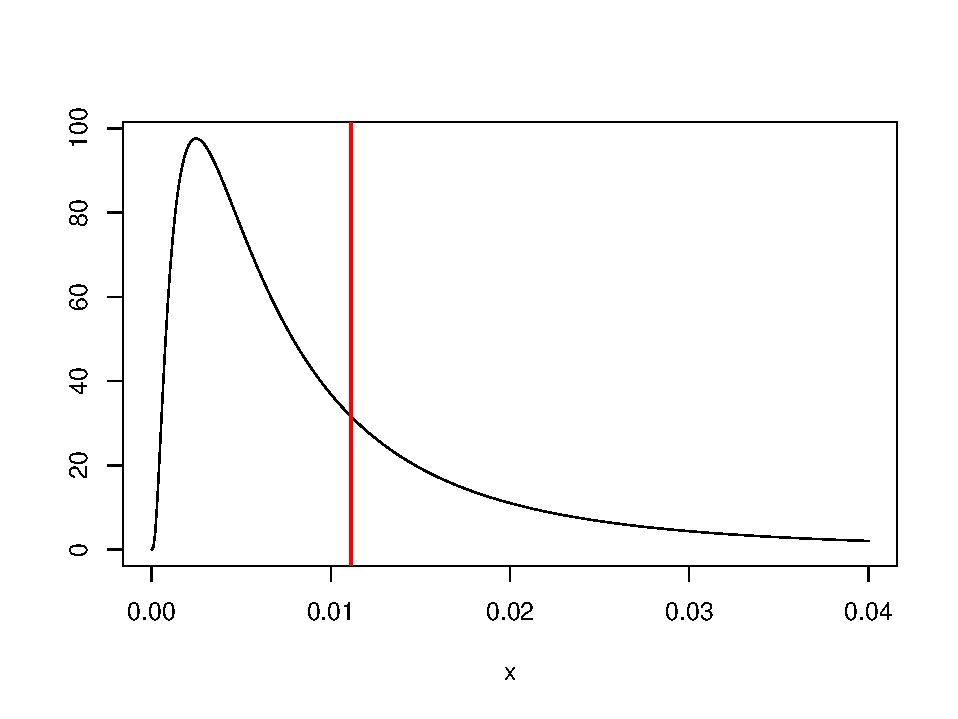
\includegraphics[width=0.75\textwidth]{figure/true.pdf}
\end{center}
\pause  This is where your individual observations $x_i$ come from.  \pause Now compare 10000 values of $\xbar$'s based on different $n$:  2, 10, 30, 75.   
\end{frame}
%------------------------------------------------------------------------------


%------------------------------------------------------------------------------
\begin{frame}
\frametitle{Example of Skew vs $n$}
For 10000 values of $\xbar$ based on samples of size \blue{$n=2$}, the\\
sampling distribution is:
\pause\begin{center}
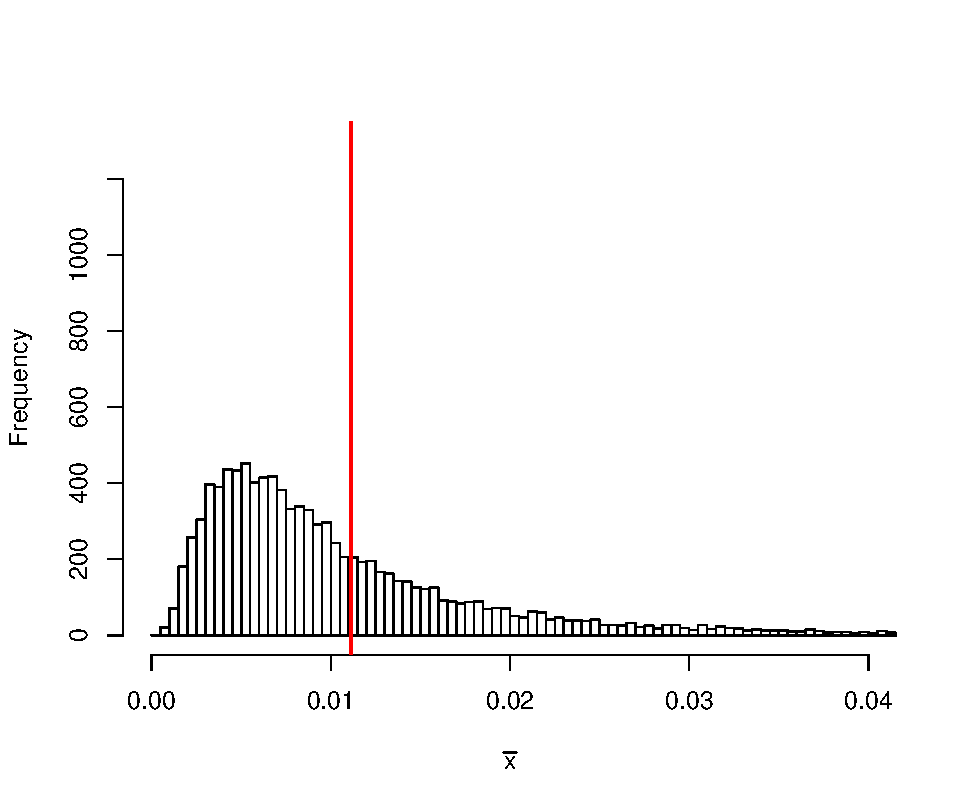
\includegraphics[width=0.8\textwidth]{figure/hist2.pdf}
\end{center}
\white{i.e. more normal and more narrow}
\end{frame}
%------------------------------------------------------------------------------


%------------------------------------------------------------------------------
\begin{frame}
\frametitle{Example of Skew vs $n$}
For 10000 values of $\xbar$ based on samples of size \blue{$n=10$}, the sampling distribution is:
\begin{center}
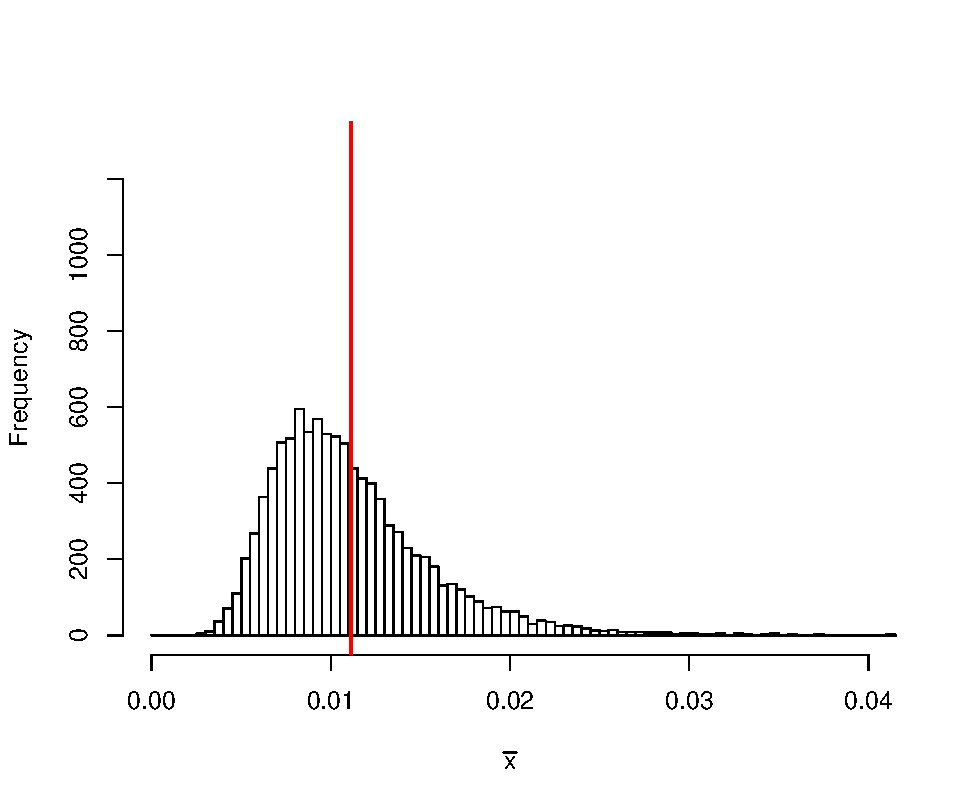
\includegraphics[width=0.8\textwidth]{figure/hist10.pdf}
\end{center}
\white{i.e. more normal and more narrow}
\end{frame}
%------------------------------------------------------------------------------


%------------------------------------------------------------------------------
\begin{frame}
\frametitle{Example of Skew vs $n$}
For 10000 values of $\xbar$ based on samples of size \blue{$n=30$}, the sampling distribution is:
\begin{center}
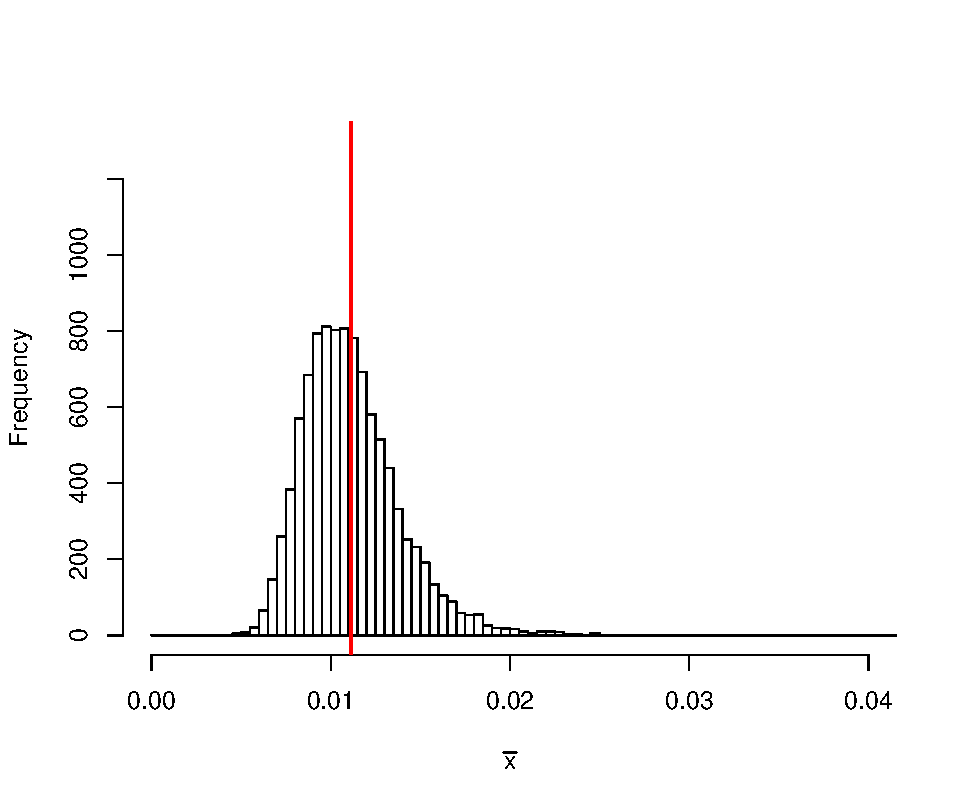
\includegraphics[width=0.8\textwidth]{figure/hist30.pdf}
\end{center}
\white{i.e. more normal and more narrow}
\end{frame}
%------------------------------------------------------------------------------


%------------------------------------------------------------------------------
\begin{frame}
\frametitle{Example of Skew vs $n$}
For 10000 values of $\xbar$ based on samples of size \blue{$n=75$}, the sampling distribution is:
\begin{center}
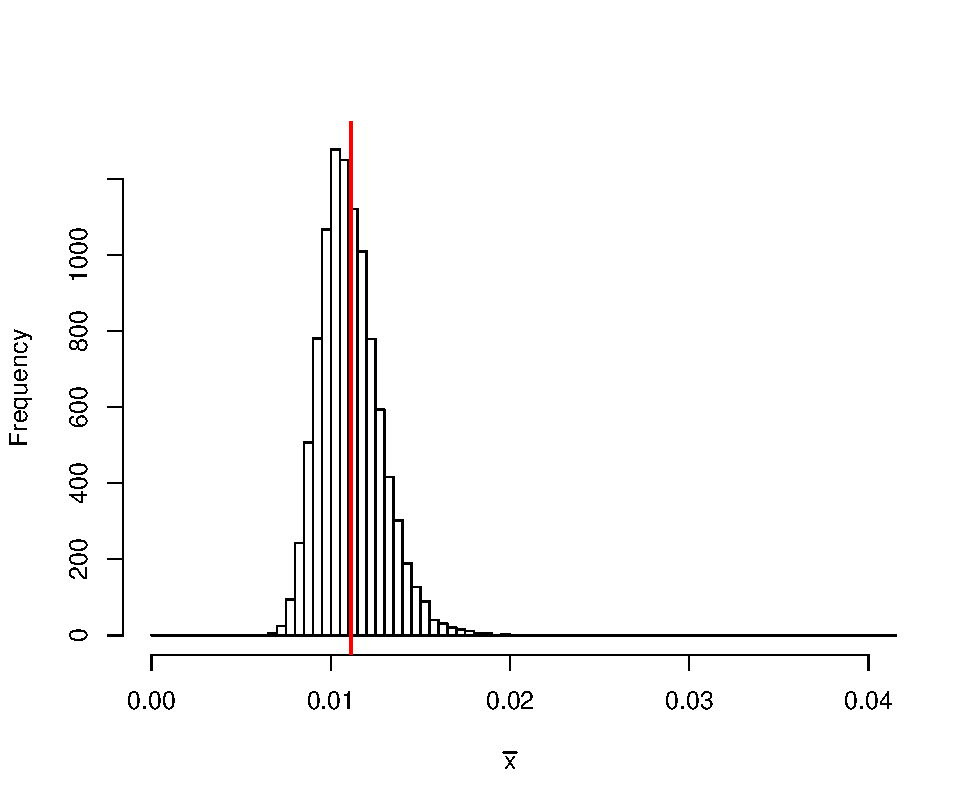
\includegraphics[width=0.8\textwidth]{figure/hist75.pdf}
\end{center}
\pause\blue{i.e. more normal and more narrow}
\end{frame}
%------------------------------------------------------------------------------


%------------------------------------------------------------------------------
\begin{frame}[fragile]
\frametitle{Intuition of a Confidence Interval}

\pause\blue{Our Goal}:  we want estimate a population parameter (e.g. $\mu$).  \pause Analogy:  imagine $\mu$ is a fish in a murky river that we want to capture:

\pause \vspace{0.25cm}

\begin{columns}
	\column{.45\textwidth} 
  Using just the point estimate:
  \column{.45\textwidth}
  Using a \blue{confidence interval}:
\end{columns}

\begin{center}

\includegraphics[height=4cm]{figure/spear.jpg}
\hspace{0.2cm}

\includegraphics[height=4cm]{figure/net.jpg}
\end{center}



\end{frame}
%------------------------------------------------------------------------------


%------------------------------------------------------------------------------
\begin{frame}[fragile]
\frametitle{Intuition of a Confidence Interval}
Recall the example of 1000 instances of $\xbar$ based on $n=100$.  Each observation came from a population distribution that was Normal with $\mu=5$ \& $\sigma=2$.  

\pause \setkeys{Gin}{width=0.4\textwidth}
\begin{center}
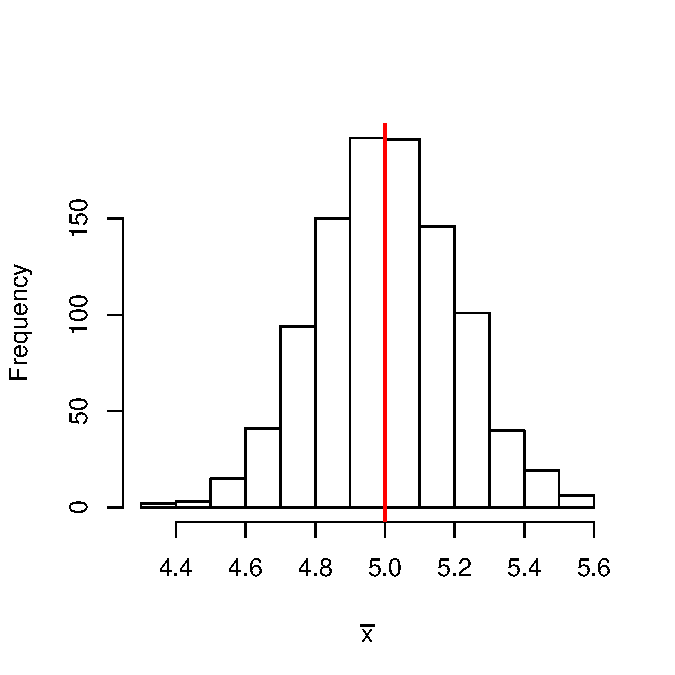
\includegraphics{figure/lec12-001}
\end{center}

\pause We observed the sampling distribution
\begin{itemize}
\item is centered at $\mu$
\item has spread $SE = \frac{\sigma}{\sqrt n} = \frac{2}{\sqrt{100}} = 0.2$
\end{itemize}

\end{frame}
%------------------------------------------------------------------------------


%------------------------------------------------------------------------------
\begin{frame}[fragile]
\frametitle{Intuition of a Confidence Interval}
A plausible range of values for the population parameter is called a \blue{confidence interval (CI)}.  Since
\begin{itemize}
\pause \item the SE is the standard deviation of the sampling distribution
\pause \item roughly 95\% of the time $\xbar$ will be within 2 SE of $\mu$ \red{if the sampling distribution is normal}
\end{itemize}

\pause If the interval spreads out 2 SE from $\xbar$, we can be roughly
\blue{``95\% confident''} that we have captured the true parameter $\mu$.  
\end{frame}
%------------------------------------------------------------------------------


%------------------------------------------------------------------------------
\begin{frame}[fragile]
\frametitle{Intuition of a Confidence Interval}
A 95\% confidence interval is (no more using rule of thumb $2 \times SD$):

\begin{eqnarray*}
\xbar \pm  1.96 SE &=& \left[\xbar - 1.96 SE, \mbox{  }\xbar + 1.96 SE\right]\\
 &=& \left[\xbar - 1.96 \frac{\sigma}{\sqrt{n}}, \mbox{  }\xbar + 1.96 \frac{\sigma}{\sqrt{n}}\right]
\end{eqnarray*}

\pause If we don't know $\sigma$, assuming the conditions hold, plug in $s$
\begin{eqnarray*}
\xbar \pm 1.96 \frac{s}{\sqrt{n}} &=& \left[\xbar - 1.96 \frac{s}{\sqrt{n}}, \mbox{  }\xbar + 1.96 \frac{s}{\sqrt{n}}\right]
\end{eqnarray*}

\end{frame}
%------------------------------------------------------------------------------


%-------------------------------------------------------------------------------
\begin{frame}
\frametitle{Confidence Intervals}

In general a confidence interval will be 
\begin{eqnarray*}
\xbar \pm z^* SE &=& \left[\xbar - z^* SE, \mbox{  }\xbar + z^* SE\right]
\end{eqnarray*}

where the \blue{critical value} $z^*$ is chosen to achieve the desired confidence.\\

\vskip 0.25cm

\pause Ex:  For 95\% confidence $z^*= 1.96$.  For 99\% confidence $z^*=2.58$

\end{frame}
%-------------------------------------------------------------------------------


%-------------------------------------------------------------------------------
\begin{frame}
\frametitle{Crucial: How to Interpret a Confidence Interval}
The confidence interval has nothing to say about any particular calculated interval; it only pertains to the \blue{method} used to construct the interval:
\vskip 0.25cm
\begin{itemize}
\pause \item\blue{Wrong, yet common, interpretation}:  There is a 95\% chance that the C.I. captures the true population mean $\mu$.  The probability is 0 or 1: either it does or it doesn't.  
%--------------------
\pause \item\blue{Correct, interpretation}:  If we were to repeat this sampling procedure 100 times, we expect 95 (i.e. 95\%) of calculated C.I.'s to capture the true $\mu$
\end{itemize}
 
\end{frame}
%-------------------------------------------------------------------------------


%-------------------------------------------------------------------------------
\begin{frame}
\frametitle{Illustration:  How to Interpret a Confidence Interval}
In Chapter 4 there is an example of finish times (in minutes) from the 2012 Cherry Blossom 10 mile run with $n=16,924$ participants.  In this case, we can compute the \blue{true} population mean $\mu=94.52$.

\vspace{0.5cm}

\pause Say we take 25 (random) samples of size $n=100$ and for each sample we compute:
\begin{itemize}
\item $\xbar$
\item $s$
\item and hence the 95\% CI:  $\left[
\overline{x} - 1.96 \times\frac{s}{\sqrt n}, \mbox{  }
\overline{x} + 1.96 \times\frac{s}{\sqrt n}
\right]$
\end{itemize}
\end{frame}
%-------------------------------------------------------------------------------


%-------------------------------------------------------------------------------
\begin{frame}
\frametitle{How to Interpret a Confidence Interval}
Of the 25 CI's based on 25 different samples of size $n=100$, one of them (in red) did not capture the true population mean $\mu$:

\begin{center}
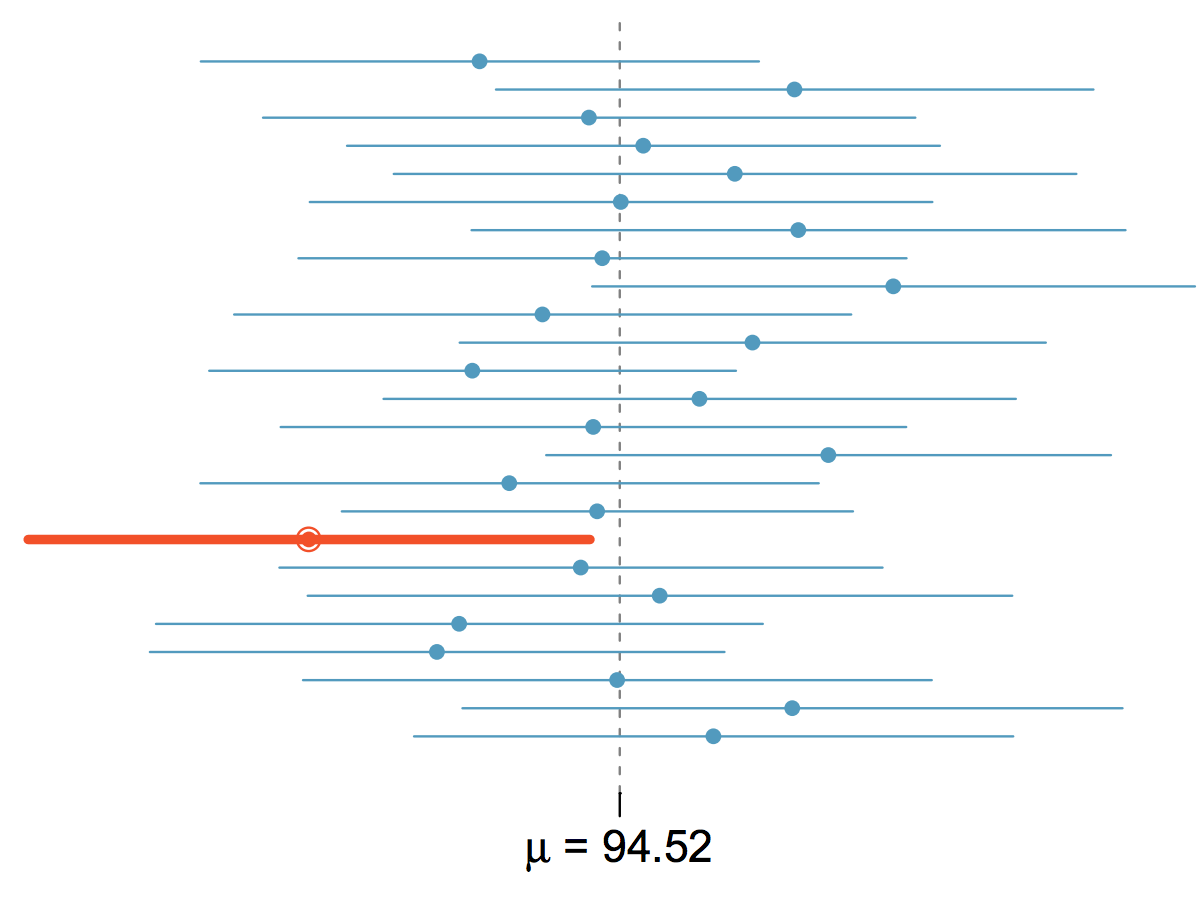
\includegraphics[width=8cm]{figure/CI.png}
\end{center}

\end{frame}
%-------------------------------------------------------------------------------


%-------------------------------------------------------------------------------
\begin{frame}
\frametitle{Political Polls}
\begin{quotation}
\noindent We polled the electorate and found that 45\% of voters plan to vote for candidate $X$.  The margin of error for this poll is $\pm 3.4$ percentage points 19 times out of 20.  
\end{quotation}
\pause What does this mean?
\begin{itemize}
\item ``19 times out of 20'' indicates 95\%
\item The margin of error of $\pm 3.4$\% indicates that 95\% C.I. is:
\[45 \pm 3.4 \% = [41.6, 48.4]\]
\end{itemize}
\pause \blue{Intrepretation}: the interpretation is not that there is a 95\% chance that $[41.6, 48.4]$ captures the true \%'age.  Rather, that if we were to take 20 such polls, 19 of them would capture the true \%'age.
\end{frame}
%-------------------------------------------------------------------------------


%------------------------------------------------------------------------------
\begin{frame}[fragile]
\frametitle{Next Time}

Hypothesis Testing:  we can perform \blue{statistical tests} on population parameters such as $\mu$:

\vspace{0.5cm}

Define:
\begin{itemize}
\item Null and alternative hypotheses.
\item Testing hypotheses using confidence intervals.
\item Types of errors
\end{itemize}

\end{frame}
%------------------------------------------------------------------------------


\end{document}




